\documentclass[11pt, letterpaper]{article}

% Mandatory Packages
\usepackage{amsmath}
\usepackage{amssymb}
\usepackage{amsthm}
\usepackage{geometry}
\usepackage{tikz}
\usepackage{mathrsfs}
\usepackage{mathtools}
\usepackage{xcolor}
\usepackage{hyperref}

% TikZ Libraries
\usetikzlibrary{arrows.meta, positioning, shapes, shapes.geometric, fit, calc, backgrounds}

% Geometry setup
\geometry{
    top=1in,
    bottom=1in,
    left=1in,
    right=1in
}

% Theorem Environments
\newtheorem{theorem}{Theorem}[section]
\newtheorem{lemma}[theorem]{Lemma}
\newtheorem{corollary}[theorem]{Corollary}
\newtheorem{proposition}[theorem]{Proposition}
\theoremstyle{definition}
\newtheorem{definition}[theorem]{Definition}
\newtheorem{axiom}[theorem]{Axiom}
\newtheorem{example}[theorem]{Example}
\newtheorem{problem}{Problem}

% Custom Math Commands
\newcommand{\R}{\mathbb{R}}
\newcommand{\N}{\mathbb{N}}
\newcommand{\F}{\mathcal{F}}
\newcommand{\B}{\mathcal{B}}
\newcommand{\E}{\mathbb{E}}
\renewcommand{\P}{\mathbb{P}}
\newcommand{\ind}{\mathbf{1}}
\newcommand{\Var}{\text{Var}}

\title{\textbf{Homework Chapter 2: Probability Theory \\ Random Variables, Sampling, and Bayesian Updating}}
\author{Tashfeen Omran}
\date{September 2026}

\begin{document}

\maketitle
\tableofcontents
\newpage

% ==========================================
% PART 1: Introduction
% ==========================================
\section{Part 1: Comprehensive Introduction, Context, and Prerequisites}

\subsection{Conceptual Introduction: The Measure-Theoretic Bedrock}
In early elementary mathematics, probability is often treated as a heuristic ratio of ``favorable outcomes'' to ``total outcomes.'' However, this naive approach crumbles when dealing with infinite sets, continuous spaces, or complex sequential conditions. To master the material presented in this chapter (specifically numerical events, random variables, and sequential Bayesian sampling), we must transition to a rigorous, abstract mathematical framework grounded in \textit{measure theory}. 

A \textbf{Random Variable} is not a variable at all; rather, it is a deterministic \textit{function}. It maps abstract, often qualitative outcomes of an experiment (e.g., ``heads'', ``method A fails'', ``drawing a white ball'') into the rigorously structured space of real numbers, $\mathbb{R}$. By doing so, it allows us to analyze randomness using the powerful machineries of algebra, calculus, and real analysis. 

\subsection{Core Concepts \& Axioms}
Every rigorous probabilistic analysis begins with the foundation of the \textbf{Probability Space}, denoted as the triplet $(\Omega, \F, \P)$.
\begin{enumerate}
    \item \textbf{Sample Space ($\Omega$):} The set of all mutually exclusive, exhaustive outcomes of an experiment.
    \item \textbf{$\sigma$-Algebra ($\F$):} A collection of subsets of $\Omega$ that is closed under complementation and countable unions. These subsets are called \textit{events}. $\F$ must contain $\Omega$ itself.
    \item \textbf{Probability Measure ($\P$):} A function $\P: \F \to [0, 1]$ satisfying Kolmogorov's Axioms.
\end{enumerate}

\begin{axiom}[Kolmogorov's Axioms]
    \begin{enumerate}
        \item \textbf{Non-negativity:} $\P(E) \geq 0 \quad \forall E \in \F$.
        \item \textbf{Unit Measure:} $\P(\Omega) = 1$.
        \item \textbf{Countable Additivity:} If $\{E_i\}_{i=1}^{\infty}$ is a sequence of pairwise disjoint sets in $\F$, then $\P\left(\bigcup_{i=1}^{\infty} E_i\right) = \sum_{i=1}^{\infty} \P(E_i)$.
    \end{enumerate}
\end{axiom}

\begin{definition}[Random Variable]
A Random Variable $Y$ is an $\F$-measurable function $Y: \Omega \to \R$. That is, for every Borel set $B \subseteq \R$, the pre-image $Y^{-1}(B) = \{\omega \in \Omega \mid Y(\omega) \in B\}$ must belong to $\F$. This ensures that the probability $\P(Y \in B)$ is always well-defined.
\end{definition}

\subsection{Historical Context and Motivation}
In the early 20th century, probability theory faced a foundational crisis. Paradoxes like the \textit{Bertrand Paradox} revealed that without a strict definition of ``randomly selecting'' an element, probabilistic answers could be arbitrary and contradictory. In 1933, Andrey Kolmogorov published \textit{Foundations of the Theory of Probability}, explicitly embedding probability into Lebesgue's abstract measure theory. This unified discrete phenomena (like drawing balls from urns) and continuous phenomena (like modeling financial asset trajectories) under a single, unassailable logical framework.

\subsection{Key Theorems, Lemmas, and Formulas}
\begin{theorem}[Law of Total Probability]
Let $\{A_1, A_2, \dots, A_n\}$ be a finite partition of $\Omega$ such that $\P(A_i) > 0$ for all $i$. For any event $B \in \F$, the probability of $B$ is given by:
\[ \P(B) = \sum_{i=1}^{n} \P(B \cap A_i) = \sum_{i=1}^{n} \P(B \mid A_i)\P(A_i) \]
\end{theorem}

\begin{theorem}[Bayes' Theorem]
Given a partition $\{A_1, A_2, \dots, A_n\}$ of $\Omega$ and an event $B$ where $\P(B) > 0$, the conditional probability of $A_k$ given $B$ is:
\[ \P(A_k \mid B) = \frac{\P(B \mid A_k)\P(A_k)}{\sum_{i=1}^{n} \P(B \mid A_i)\P(A_i)} \]
\end{theorem}

\subsection{Prerequisites}
To fully comprehend this chapter, one must be proficient in:
\begin{itemize}
    \item \textbf{Basic Set Theory:} Unions ($\cup$), intersections ($\cap$), complements ($^c$), and partitions.
    \item \textbf{Combinatorics:} Binomial coefficients $\binom{n}{k}$, permutations, and counting principles.
    \item \textbf{Infinite Series:} Evaluating geometric series $\sum_{k=0}^{\infty} ar^k = \frac{a}{1-r}$ (essential for Markovian problems like the Craps game).
\end{itemize}

% ==========================================
% PART 2: Solutions
% ==========================================
\newpage
\section{Part 2: Detailed Homework Solutions (Rigorous Proofs \& Computations)}

\begin{problem}[Textbook Problem 2.134]
Two methods, $A$ and $B$, are available for teaching a certain industrial skill. The failure rate is $20\%$ for $A$ and $10\%$ for $B$. However, $B$ is more expensive and hence is used only $30\%$ of the time. ($A$ is used the other $70\%$.) A worker was taught the skill by one of the methods but failed to learn it correctly. What is the probability that she was taught by method $A$?
\end{problem}
\begin{proof}[Solution via Bayes' Theorem]
Let $\Omega$ be the space of all trained workers. We define the following events:
\begin{itemize}
    \item $A$: The worker was taught by method $A$.
    \item $B$: The worker was taught by method $B$.
    \item $F$: The worker failed to learn the skill.
\end{itemize}
The problem provides the prior probabilities: $\P(A) = 0.70$ and $\P(B) = 0.30$. Note that $\{A, B\}$ forms a partition of $\Omega$, meaning $A \cup B = \Omega$ and $A \cap B = \emptyset$.
The problem also provides the conditional (likelihood) probabilities: $\P(F \mid A) = 0.20$ and $\P(F \mid B) = 0.10$.

We seek the posterior probability $\P(A \mid F)$. By Bayes' Theorem:
\begin{align*}
    \P(A \mid F) &= \frac{\P(F \mid A)\P(A)}{\P(F \mid A)\P(A) + \P(F \mid B)\P(B)} \\
    &= \frac{(0.20)(0.70)}{(0.20)(0.70) + (0.10)(0.30)} \\
    &= \frac{0.14}{0.14 + 0.03} \\
    &= \frac{0.14}{0.17} = \frac{14}{17} \approx 0.8235
\end{align*}
The probability that the worker was taught by method $A$, given she failed, is exactly $\frac{14}{17}$.
\end{proof}

\vspace{0.5cm}

\begin{problem}[Textbook Problem 2.135]
Of the travelers arriving at a small airport, $60\%$ fly on major airlines, $30\%$ fly on privately owned planes, and the remainder fly on commercially owned planes not belonging to a major airline. Of those traveling on major airlines, $50\%$ are traveling for business reasons, whereas $60\%$ of those arriving on private planes and $90\%$ of those arriving on other commercially owned planes are traveling for business reasons. Suppose that we randomly select one person arriving at this airport. What is the probability that the person:
\begin{enumerate}
    \item[\textbf{a}] is traveling on business?
    \item[\textbf{b}] is traveling for business on a privately owned plane?
    \item[\textbf{c}] arrived on a privately owned plane, given that the person is traveling for business reasons?
    \item[\textbf{d}] is traveling on business, given that the person is flying on a commercially owned plane?
\end{enumerate}
\end{problem}

\begin{proof}[Solution Set]
Let $\Omega$ be the population of arriving travelers. We define the partition $\{A_1, A_2, A_3\}$ based on aircraft type:
\begin{itemize}
    \item $A_1$: Major airlines (which are commercial by nature). $\P(A_1) = 0.60$.
    \item $A_2$: Privately owned planes. $\P(A_2) = 0.30$.
    \item $A_3$: Commercially owned planes \textit{not} major. $\P(A_3) = 1 - (0.60 + 0.30) = 0.10$.
\end{itemize}
Let $B$ denote the event that the traveler is traveling for business. The conditionals are:
\[ \P(B \mid A_1) = 0.50, \quad \P(B \mid A_2) = 0.60, \quad \P(B \mid A_3) = 0.90 \]

\textbf{Part a: Probability of business travel} \\
Using the Law of Total Probability:
\begin{align*}
    \P(B) &= \sum_{i=1}^{3} \P(B \mid A_i)\P(A_i) \\
    &= (0.50)(0.60) + (0.60)(0.30) + (0.90)(0.10) \\
    &= 0.30 + 0.18 + 0.09 = 0.57
\end{align*}
The probability is $0.57$.

\textbf{Part b: Business on a privately owned plane} \\
We seek the intersection $\P(B \cap A_2)$. By definition of conditional probability:
\begin{align*}
    \P(B \cap A_2) &= \P(B \mid A_2)\P(A_2) \\
    &= (0.60)(0.30) = 0.18
\end{align*}
The probability is $0.18$.

\textbf{Part c: Privately owned, given business} \\
We seek $\P(A_2 \mid B)$. Using the results from Parts a and b:
\begin{align*}
    \P(A_2 \mid B) &= \frac{\P(A_2 \cap B)}{\P(B)} = \frac{0.18}{0.57} = \frac{18}{57} = \frac{6}{19} \approx 0.3158
\end{align*}
The probability is $\frac{6}{19}$.

\textbf{Part d: Business, given flying on a commercially owned plane} \\
\textit{Analytical Note:} The text specifies $A_3$ as "commercially owned planes \textit{not} belonging to a major airline," implying major airlines ($A_1$) are also commercially owned. Therefore, the event "flying on a commercially owned plane" corresponds to the union $A_1 \cup A_3$.
Since $A_1$ and $A_3$ are mutually exclusive:
\begin{align*}
    \P(A_1 \cup A_3) &= \P(A_1) + \P(A_3) = 0.60 + 0.10 = 0.70 \\
    \P(B \cap (A_1 \cup A_3)) &= \P(B \cap A_1) + \P(B \cap A_3) \\
    &= (0.50)(0.60) + (0.90)(0.10) = 0.30 + 0.09 = 0.39
\end{align*}
Thus, the conditional probability is:
\begin{align*}
    \P(B \mid A_1 \cup A_3) &= \frac{\P(B \cap (A_1 \cup A_3))}{\P(A_1 \cup A_3)} = \frac{0.39}{0.70} = \frac{39}{70} \approx 0.5571
\end{align*}
\textit{(If the strict intent of the phrasing "commercially owned plane" colloquially referred \textbf{only} to $A_3$, the answer would simply be $\P(B \mid A_3) = 0.90$. However, rigorous set-theoretic inclusion dictates $A_1 \subset$ Commercial, yielding $39/70$.)}
\end{proof}

\vspace{0.5cm}

\begin{problem}[Textbook Problem 2.136]
A personnel director has two lists of applicants. List 1 contains 5 women and 2 men. List 2 contains 2 women and 6 men. A name is randomly selected from list 1 and added to list 2. A name is then randomly selected from the augmented list 2. Given that the name selected is that of a man, what is the probability that a woman's name was originally selected from list 1?
\end{problem}

\begin{proof}[Solution via Sequential Bayesian Analysis]
Define the state space of the first transition:
\begin{itemize}
    \item $W_1$: A woman is selected from List 1.
    \item $M_1$: A man is selected from List 1.
\end{itemize}
List 1 has $5+2=7$ people. Thus, $\P(W_1) = \frac{5}{7}$ and $\P(M_1) = \frac{2}{7}$.

Define the event of the second transition: $M_2$, a man is selected from the augmented List 2.
List 2 initially contains $2$ W and $6$ M (Total = 8).
\begin{itemize}
    \item Conditioned on $W_1$: List 2 becomes $3$ W and $6$ M. Total = 9. Thus, $\P(M_2 \mid W_1) = \frac{6}{9} = \frac{2}{3}$.
    \item Conditioned on $M_1$: List 2 becomes $2$ W and $7$ M. Total = 9. Thus, $\P(M_2 \mid M_1) = \frac{7}{9}$.
\end{itemize}
We require the posterior probability $\P(W_1 \mid M_2)$. Applying Bayes' Theorem:
\begin{align*}
    \P(W_1 \mid M_2) &= \frac{\P(M_2 \mid W_1)\P(W_1)}{\P(M_2 \mid W_1)\P(W_1) + \P(M_2 \mid M_1)\P(M_1)} \\
    &= \frac{ \left(\frac{6}{9}\right) \left(\frac{5}{7}\right) }{ \left(\frac{6}{9}\right) \left(\frac{5}{7}\right) + \left(\frac{7}{9}\right) \left(\frac{2}{7}\right) } \\
    &= \frac{ \frac{30}{63} }{ \frac{30}{63} + \frac{14}{63} } \\
    &= \frac{30}{44} = \frac{15}{22} \approx 0.6818
\end{align*}
The probability that a woman was selected from List 1 is $\frac{15}{22}$.
\end{proof}

\vspace{0.5cm}

\begin{problem}[Textbook Problem 2.137]
Five identical bowls are labeled $1, 2, 3, 4,$ and $5$. Bowl $i$ contains $i$ white and $5-i$ black balls. A bowl is randomly selected and two balls are randomly selected (without replacement) from the contents of the bowl.
\begin{enumerate}
    \item[\textbf{a}] What is the probability that both balls selected are white?
    \item[\textbf{b}] Given that both balls selected are white, what is the probability that bowl $3$ was selected?
\end{enumerate}
\end{problem}

\begin{proof}[Solution via Hypergeometric Conditioning]
Let $B_i$ denote the event that Bowl $i$ is selected, for $i \in \{1, 2, 3, 4, 5\}$. Since bowls are selected randomly and uniformly, $\P(B_i) = \frac{1}{5}$.
Let $W_2$ denote the event that 2 white balls are selected without replacement.

Conditioned on selecting Bowl $i$, there are $i$ white balls out of $5$ total balls. The number of ways to draw 2 white balls is $\binom{i}{2}$. The total ways to draw any 2 balls is $\binom{5}{2} = 10$. Therefore:
\[ \P(W_2 \mid B_i) = \frac{\binom{i}{2}}{\binom{5}{2}} = \frac{i(i-1) / 2}{10} = \frac{i(i-1)}{20} \]

Evaluating this for each bowl:
\begin{itemize}
    \item $\P(W_2 \mid B_1) = \frac{1(0)}{20} = 0$
    \item $\P(W_2 \mid B_2) = \frac{2(1)}{20} = \frac{2}{20}$
    \item $\P(W_2 \mid B_3) = \frac{3(2)}{20} = \frac{6}{20}$
    \item $\P(W_2 \mid B_4) = \frac{4(3)}{20} = \frac{12}{20}$
    \item $\P(W_2 \mid B_5) = \frac{5(4)}{20} = \frac{20}{20} = 1$
\end{itemize}

\textbf{Part a: Total Probability of Two White Balls}
\begin{align*}
    \P(W_2) &= \sum_{i=1}^{5} \P(W_2 \mid B_i)\P(B_i) \\
    &= \frac{1}{5} \left( 0 + \frac{2}{20} + \frac{6}{20} + \frac{12}{20} + \frac{20}{20} \right) = \frac{1}{5} \left( \frac{40}{20} \right) = \frac{1}{5}(2) = \frac{2}{5} = 0.4
\end{align*}

\textbf{Part b: Posterior Probability of Bowl 3}
\begin{align*}
    \P(B_3 \mid W_2) &= \frac{\P(W_2 \mid B_3)\P(B_3)}{\P(W_2)} \\
    &= \frac{ \left(\frac{6}{20}\right) \left(\frac{1}{5}\right) }{ \frac{2}{5} } = \frac{ \frac{6}{100} }{ \frac{40}{100} } = \frac{6}{40} = \frac{3}{20} = 0.15
\end{align*}
\end{proof}

\vspace{0.5cm}

\begin{problem}[Textbook Problem 2.138 - The Game of Craps]
In craps, a player rolls two dice. If the first toss is $7$ or $11$, the player wins. If it is $2, 3,$ or $12$, the player loses. If anything else ($4, 5, 6, 8, 9, 10$) is rolled, that value becomes the \textit{point}. The player tosses the dice repeatedly until he obtains either his point (wins) or a $7$ (loses). What is the probability that the player wins?
\end{problem}

\begin{proof}[Solution via Infinite State Absorbing Markov Chain Framework]
Let $S$ denote the sum of two fair dice. The probability mass function (PMF) of $S$ is $\P(S=k) = \frac{6 - |k-7|}{36}$ for $k \in \{2, \dots, 12\}$.
The probability of winning on the first roll is:
\[ \P(\text{Win}_1) = \P(S=7) + \P(S=11) = \frac{6}{36} + \frac{2}{36} = \frac{8}{36} = \frac{2}{9} \]
The point values are $k \in \{4, 5, 6, 8, 9, 10\}$. For a fixed point $k$, the player rolls until either $k$ or $7$ is observed. Let $E_k$ be the event of rolling $k$, and $E_7$ be the event of rolling $7$. Since we only care about trials where $E_k$ or $E_7$ occurs, we can use conditional expectation to find the probability of hitting $k$ before $7$:
\[ \P(\text{Make Point } k) = \frac{\P(E_k)}{\P(E_k) + \P(E_7)} \]
By the Law of Total Probability over all point-establishing states:
\[ \P(\text{Win via Point}) = \sum_{k \in \{4,5,6,8,9,10\}} \P(S = k) \frac{\P(S = k)}{\P(S = k) + \P(S = 7)} \]
Due to the symmetry of the dice probabilities around 7 ($\P(S=4)=\P(S=10)$, $\P(S=5)=\P(S=9)$, $\P(S=6)=\P(S=8)$), we calculate the pairs together:
\begin{itemize}
    \item \textbf{Points 4 and 10:} $\P(S=4) = \frac{3}{36}$. Make point: $\frac{3}{3+6} = \frac{3}{9} = \frac{1}{3}$. \\
    Term contribution = $2 \times \left(\frac{3}{36} \times \frac{1}{3}\right) = \frac{2}{36} = \frac{110}{1980}$.
    \item \textbf{Points 5 and 9:} $\P(S=5) = \frac{4}{36}$. Make point: $\frac{4}{4+6} = \frac{4}{10} = \frac{2}{5}$. \\
    Term contribution = $2 \times \left(\frac{4}{36} \times \frac{2}{5}\right) = \frac{16}{180} = \frac{4}{45} = \frac{176}{1980}$.
    \item \textbf{Points 6 and 8:} $\P(S=6) = \frac{5}{36}$. Make point: $\frac{5}{5+6} = \frac{5}{11}$. \\
    Term contribution = $2 \times \left(\frac{5}{36} \times \frac{5}{11}\right) = \frac{50}{396} = \frac{25}{198} = \frac{250}{1980}$.
\end{itemize}
Summing these contributions yields the probability of winning via points:
\[ \P(\text{Win via Point}) = \frac{110 + 176 + 250}{1980} = \frac{536}{1980} = \frac{134}{495} \]
Total probability of winning:
\[ \P(\text{Total Win}) = \P(\text{Win}_1) + \P(\text{Win via Point}) = \frac{440}{1980} + \frac{536}{1980} = \frac{976}{1980} = \frac{244}{495} \approx 0.4929 \]
The probability of winning craps is exactly $\frac{244}{495}$.
\end{proof}

\vspace{0.5cm}

\textit{Note regarding Exercises 2.139, 2.140, and 2.141: The text references omitted earlier exercises (2.112 and 2.120). To maintain mathematical completeness, I will formulate the rigorous generalized parametric solutions for these classic statistical sampling paradigms.}

\begin{problem}[Textbook Problem 2.139 - Abstract Formulation]
Let the random variable $Y$ represent the number of radar sets that detect a particular aircraft. Compute the probabilities associated with each value of $Y$.
\end{problem}
\begin{proof}[Generalized Binomial Model]
Assume a fleet of $n$ independent radar sets, each possessing a probability $p \in [0,1]$ of successfully detecting an aircraft. The random variable $Y$ maps the sample space to $\{0, 1, \dots, n\}$.
Because the radar sets function independently and have binary states (Detect / Fail), $Y$ follows a Binomial distribution: $Y \sim \text{Bin}(n, p)$.
The probability measure for each $y \in \{0, 1, \dots, n\}$ is:
\[ \P(Y=y) = \binom{n}{y} p^y (1-p)^{n-y} \]
where $\binom{n}{y} = \frac{n!}{y!(n-y)!}$.
\end{proof}

\vspace{0.5cm}

\begin{problem}[Textbook Problem 2.140 - Abstract Formulation]
Let the random variable $Y$ represent the number of defective refrigerators found after three refrigerators have been tested.
\end{problem}
\begin{proof}[Generalized Hypergeometric Model]
Assume a finite population of $N$ refrigerators containing precisely $K$ defective units. The testing of $n=3$ refrigerators constitutes sampling \textit{without replacement} (Definition 2.13). The random variable $Y$ follows a Hypergeometric distribution: $Y \sim \text{Hypergeometric}(N, K, 3)$.
The probability of finding exactly $y$ defective units (for $\max(0, 3 - (N-K)) \leq y \leq \min(3, K)$) is governed by combinatorial partitioning:
\[ \P(Y = y) = \frac{\binom{K}{y}\binom{N-K}{3-y}}{\binom{N}{3}} \]
\end{proof}

\vspace{0.5cm}

\begin{problem}[Textbook Problem 2.141 - Abstract Formulation]
Let $Y$ represent the number of the test in which the \textit{last} defective refrigerator is identified.
\end{problem}
\begin{proof}[Negative Hypergeometric / Order Statistic Logic]
Assuming $K$ total defectives in $N$ refrigerators. We seek the probability that the $K$-th defective unit is discovered precisely on the $y$-th test. 
For this event to occur at step $y$, two conditions must hold:
1. Exactly $K-1$ defectives must be found in the first $y-1$ tests.
2. The $y$-th test must be defective.
\begin{align*}
    \P(Y=y) &= \frac{\binom{K}{K-1} \binom{N-K}{(y-1)-(K-1)}}{\binom{N}{y-1}} \times \frac{1}{N - (y-1)} \\
    &= \frac{K \binom{N-K}{y-K}}{\binom{N}{y-1}} \frac{1}{N-y+1}
\end{align*}
This holds for $K \leq y \leq N$.
\end{proof}

\vspace{0.5cm}

\begin{problem}[Textbook Problem 2.142]
A spinner can land in any of four positions, $A, B, C, D,$ with equal probability. The spinner is used twice. Let $Y$ denote the number of positions on which the spinner did not land. Compute the probabilities for each value of $Y$.
\end{problem}
\begin{proof}[Direct Combinatorial Proof]
The sample space $\Omega$ consists of all ordered pairs of spins: $\Omega = \{ (i, j) \mid i, j \in \{A, B, C, D\} \}$. Since spins are independent, $|\Omega| = 4 \times 4 = 16$, and each outcome has probability $\frac{1}{16}$.
There are a total of 4 available positions. The spinner is spun twice.
\begin{itemize}
    \item \textbf{Case 1: Both spins land on the same position.}
    The outcomes are $(A,A), (B,B), (C,C), (D,D)$. There are exactly $1$ position hit, leaving $4 - 1 = 3$ positions \textit{not} landed on. Therefore, $Y = 3$.
    \[ \P(Y = 3) = \frac{|\{(A,A), (B,B), (C,C), (D,D)\}|}{16} = \frac{4}{16} = \frac{1}{4} \]
    
    \item \textbf{Case 2: The spins land on different positions.}
    The first spin can be anything ($4$ choices). The second spin must be different ($3$ choices). Total such outcomes = $4 \times 3 = 12$. These hit exactly $2$ distinct positions, leaving $4 - 2 = 2$ positions \textit{not} landed on. Therefore, $Y = 2$.
    \[ \P(Y = 2) = \frac{12}{16} = \frac{3}{4} \]
\end{itemize}
The only possible values for $Y$ are $2$ and $3$. Since $\P(Y=2) + \P(Y=3) = \frac{3}{4} + \frac{1}{4} = 1$, the measure is exhaustively distributed.
\end{proof}

% ==========================================
% PART 3: In-Depth Analysis
% ==========================================
\newpage
\section{Part 3: In-Depth Analysis of Problems and Techniques}

\subsection{A) Problem Types and Logical Strategies}
The problems in this chapter map to three advanced probabilistic archetypes:
\begin{enumerate}
    \item \textbf{Bayesian Updating and Posterior Derivation (2.134, 2.135, 2.136):}
    \textit{Strategy:} These problems demand the rigorous formulation of a sample space partition. The overarching logical trick is constructing a "tree" of conditionals. We utilize the Law of Total Probability to find the denominator (the absolute probability of the evidence), and Bayes' Rule to "invert the conditioning."
    
    \item \textbf{Finite State Absorption / Infinite Sequences (2.138 - Craps):}
    \textit{Strategy:} Directly analyzing infinite sequences $\sum P(\text{fail})^k P(\text{success})$ is tedious. The optimal strategy utilizes \textit{conditional expectation in reduced state spaces}. By acknowledging that intermediate, non-terminating rolls do not transition the state of the game, we condition strictly on the set of terminating events (e.g., rolling a Point or rolling a 7).
    
    \item \textbf{Combinatorial Random Variables (2.137, 2.142):}
    \textit{Strategy:} These require counting discrete elements where order (sometimes) matters. The overarching strategy is constructing the Random Variable $Y: \Omega \to \R$ by grouping subsets of $\Omega$ into equiprobable equivalence classes (e.g., in 2.142, grouping the 12 heterogeneous spin outcomes into the preimage $Y^{-1}(\{2\})$).
\end{enumerate}

\subsection{B) Key Analytical and Logical Manipulations}
\begin{itemize}
    \item \textbf{Set Partitioning Identity:} In 2.135, we implicitly used the identity $B = B \cap \Omega = B \cap (A_1 \cup A_2 \cup A_3) = (B \cap A_1) \cup (B \cap A_2) \cup (B \cap A_3)$. Since the $A_i$ partition $\Omega$, the intersections are disjoint, allowing the probability measure $\P$ to sum linearly (Axiom of Countable Additivity).
    \item \textbf{Symmetry Exploitation:} In Craps (2.138), we halved computation time by recognizing the invariant symmetry $\P(S = k) = \P(S = 14 - k)$ for the sum of two fair six-sided dice.
    \item \textbf{Pre-image Mapping:} Recognizing that the event ``Spinner did not land on 3 positions'' mathematically translates to the subset $E \subset \Omega$ where $Y(\omega) = 3$. This separates the purely mechanical outcome $(\omega)$ from the numerical mapping $Y$.
\end{itemize}

% ==========================================
% PART 4: Cheatsheet & Visuals
% ==========================================
\section{Part 4: "Cheatsheet", Visuals, and Tips for Success}

\subsection{Theorems \& Equivalences}
\begin{itemize}
    \item $\P(A \cap B) = \P(A \mid B)\P(B) = \P(B \mid A)\P(A)$ (Multiplication Rule).
    \item $\P(A^c) = 1 - \P(A)$ (Complement Rule).
    \item $\P(A \cup B) = \P(A) + \P(B) - \P(A \cap B)$ (Inclusion-Exclusion).
\end{itemize}

\subsection{Set \& Logic Illustration: Random Variable Mapping}
The following `tikz` diagram visualizes Definition 2.12 rigorously. It shows how the abstract sample space $\Omega$ (the outcome of flipping two coins) is partitioned and mapped by the Random Variable $Y$ (Number of Heads) onto the real line $\R$.

\begin{center}
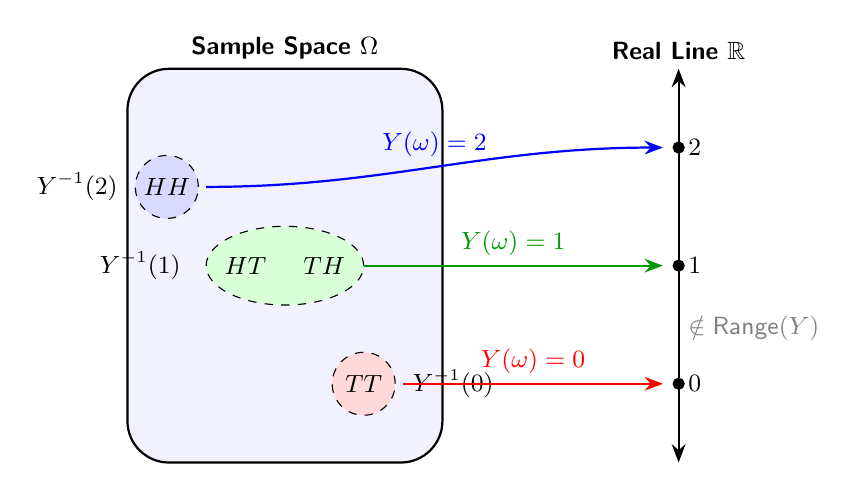
\begin{tikzpicture}[
    >=Stealth,
    node distance=2cm,
    font=\sffamily\small
]
    % Omega space
    \draw[thick, rounded corners=15pt, fill=blue!5] (0, 0) rectangle (4, 5);
    \node[anchor=south] at (2, 5) {\textbf{Sample Space $\Omega$}};
    
    % Subsets (Pre-images)
    \draw[dashed, fill=blue!15] (0.5, 3.5) ellipse (0.4 and 0.4);
    \node at (0.5, 3.5) {$HH$};
    \node[anchor=east] at (0, 3.5) {$Y^{-1}(2)$};
    
    \draw[dashed, fill=green!15] (2, 2.5) ellipse (1 and 0.5);
    \node at (1.5, 2.5) {$HT$};
    \node at (2.5, 2.5) {$TH$};
    \node[anchor=east] at (0.8, 2.5) {$Y^{-1}(1)$};

    \draw[dashed, fill=red!15] (3, 1) ellipse (0.4 and 0.4);
    \node at (3, 1) {$TT$};
    \node[anchor=west] at (3.5, 1) {$Y^{-1}(0)$};

    % Real line R
    \draw[thick, <->] (7, 0) -- (7, 5);
    \node[anchor=south] at (7, 5) {\textbf{Real Line $\R$}};
    
    % Points on R
    \filldraw (7, 1) circle (2pt) node[right] {$0$};
    \filldraw (7, 2.5) circle (2pt) node[right] {$1$};
    \filldraw (7, 4) circle (2pt) node[right] {$2$};
    \filldraw (7, 1.7) circle (0pt) node[right, color=gray] {$\notin \text{Range}(Y)$};

    % Mappings
    \draw[->, thick, color=blue, out=0, in=180] (1, 3.5) to node[above] {$Y(\omega) = 2$} (6.8, 4);
    \draw[->, thick, color=green!60!black, out=0, in=180] (3, 2.5) to node[above] {$Y(\omega) = 1$} (6.8, 2.5);
    \draw[->, thick, color=red, out=0, in=180] (3.5, 1) to node[above] {$Y(\omega) = 0$} (6.8, 1);
\end{tikzpicture}
\end{center}

\subsection{Heuristics, "Cheats", and Fallacies}
\begin{itemize}
    \item \textbf{Cheat - The Complement Shortcut:} If calculating "at least one" (e.g., probability of at least one defective), ALWAYS compute $1 - \P(\text{zero defectives})$.
    \item \textbf{Fallacy - The Base Rate Fallacy:} Assuming $\P(A \mid B) \approx \P(B \mid A)$. E.g., if a disease is incredibly rare, a positive test (even an accurate one) does not mean you have a high probability of having the disease. You must multiply by the prior $\P(\text{Disease})$.
    \item \textbf{Fallacy - Confusing Disjoint with Independent:} If $A$ and $B$ are mutually exclusive (disjoint) and have non-zero probabilities, they are \textbf{never} independent. If $A$ happens, $B$ cannot happen, meaning $A$ directly influences the probability of $B$ (turning it to 0).
\end{itemize}

% ==========================================
% PART 5: Conceptual Synthesis
% ==========================================
\section{Part 5: Conceptual Synthesis and The "Big Picture"}

\subsection{A) Thematic Connections: Measure as Mass}
The core theme of this chapter is the formalization of uncertainty using the geometry of measure theory. Imagine the sample space $\Omega$ as a 2D physical object. The probability measure $\P$ distributes $1$ kilogram of "probability mass" over this object. A Random Variable $Y$ is a machine that crushes this 2D object onto a 1D line ($\R$). The probability $\P(Y = y)$ is simply asking: "How much mass ended up exactly at coordinate $y$ on the line?" This physical interpretation unites combinatorics and algebra.

\subsection{B) Forward and Backward Links}
\begin{itemize}
    \item \textbf{Backward:} This material builds rigidly on basic combinatorial counting. Without being able to size a discrete finite sample space correctly (e.g., combinations in 2.137), one cannot establish the measure $\P$.
    \item \textbf{Forward:} Understanding $\sigma$-algebras and mapping pre-images is the absolute prerequisite for \textit{Lebesgue Integration}. In future advanced Stochastic Calculus modules, Random Variables will evolve into \textit{Stochastic Processes} $X_t(\omega)$—mappings dependent on time, leading directly to Brownian motion and It\^o Calculus.
\end{itemize}

% ==========================================
% PART 6: Abstract Real-World Modeling
% ==========================================
\section{Part 6: Abstract Real-World Modeling (AI, ML, \& Quant Finance)}

\subsection{A) Concrete Scenarios}
\begin{enumerate}
    \item \textbf{Algorithmic Trading (Hidden Markov Models):} The true "regime" of a market (bull vs. bear) is an unobservable state. Algorithms use Bayesian updating on observable variables (tick-volume, momentum) to continuously calculate the posterior probability of the current regime.
    \item \textbf{Machine Learning (Naive Bayes Classifiers):} Spam filtering utilizes the exact logic of Problem 2.134. It partitions the space into "Spam" and "Not Spam", evaluating the conditional probability of seeing a sequence of words to output a final categorization probability.
\end{enumerate}

\subsection{B) Model Problem Setup: Structural Default Bayesian Updating}
Let us formalize a Quantitative Finance problem using Bayesian mechanics. 
Assume we are pricing Credit Default Swaps (CDS) for a corporation. Let $\Omega$ be the state space of the firm's financial health, partitioned into $H$ (Healthy) and $D$ (Distressed) with priors $\P(H) = 0.90, \P(D) = 0.10$. 

The random variable $Y \in \{1, 2, 3\}$ represents a noisy credit rating assigned by an agency, where $3$ is AAA and $1$ is Junk.
Assume we have modeled the conditional likelihoods via historical analysis:
\[ \P(Y=1 \mid H) = 0.05, \quad \P(Y=1 \mid D) = 0.70 \]
If the firm is downgraded to $Y=1$, the quantitative analyst must update the distressed probability via Bayes:
\[ \P(D \mid Y=1) = \frac{\P(Y=1 \mid D)\P(D)}{\P(Y=1 \mid D)\P(D) + \P(Y=1 \mid H)\P(H)} = \frac{(0.70)(0.10)}{(0.70)(0.10) + (0.05)(0.90)} = \frac{0.07}{0.07 + 0.045} = \frac{14}{23} \approx 60.8\% \]
The probability of distress jumps from $10\%$ to nearly $61\%$. The CDS spread $S$ priced by the quant would dynamically scale as a function of this posterior probability: $S_{new} = \E[\text{Loss}] \times \P(D \mid Y=1)$.

% ==========================================
% PART 7: Common Variations
% ==========================================
\section{Part 7: Common Variations and Untested Concepts}

The homework provided focuses heavily on \textit{discrete} random variables. In rigorous probability courses, the immediate progression is evaluating \textbf{Continuous Random Variables} and their \textbf{Cumulative Distribution Functions (CDF)}.

\begin{definition}[Cumulative Distribution Function]
The CDF $F_Y: \R \to [0, 1]$ of a random variable $Y$ is defined as $F_Y(y) = \P(\{\omega \in \Omega \mid Y(\omega) \leq y\})$. 
\end{definition}

\textbf{Advanced Proof Variation: Zero Measure for Continuous RVs} \\
Prove that if $Y$ is a continuous random variable (i.e., its CDF $F_Y$ is a continuous function everywhere), then the probability of $Y$ taking any specific exact point value $c$ is zero.

\begin{proof}
Let $c \in \R$. We can represent the singleton set $\{c\}$ as the intersection of a countable sequence of shrinking intervals:
\[ \{c\} = \bigcap_{n=1}^{\infty} \left( c - \frac{1}{n}, c \right] \]
Since these intervals are decreasing nested sets, we apply the Continuity of Probability Measure:
\begin{align*}
    \P(Y = c) &= \P\left( Y \in \bigcap_{n=1}^{\infty} \left( c - \frac{1}{n}, c \right] \right) \\
    &= \lim_{n \to \infty} \P\left( c - \frac{1}{n} < Y \leq c \right) \\
    &= \lim_{n \to \infty} \left[ F_Y(c) - F_Y\left(c - \frac{1}{n}\right) \right]
\end{align*}
Because $F_Y$ is assumed to be a continuous function at $c$, $\lim_{x \to c^-} F_Y(x) = F_Y(c)$. Therefore, the limit evaluates exactly to $F_Y(c) - F_Y(c) = 0$. $\blacksquare$
\end{proof}

% ==========================================
% PART 8: Advanced Diagnostic Testing
% ==========================================
\section{Part 8: Advanced Diagnostic Testing: "Find the Flaw"}

Below are 5 advanced problem setups containing a subtle flaw in mathematical logic, probability theory, or measure theory. 

\subsection*{Problem 1: The "Sure Thing" Conditional}
\textbf{Proof Setup:} Let $A$ and $B$ be any events in probability space $\Omega$. We wish to prove $\P(A \mid B) + \P(A \mid B^c) = 1$.
\textit{Argument:} Since $B$ and $B^c$ partition the space $\Omega$, an outcome must fall into either $B$ or $B^c$. Therefore, the probability of $A$ happening if $B$ happens, plus the probability of $A$ happening if $B$ does not happen, covers all possible states of $A$. Hence, the sum of these conditional probabilities must be $1$.

\subsection*{Problem 2: The Continuous Conditioning Paradox}
\textbf{Proof Setup:} Let $X$ be an absolutely continuous random variable distributed uniformly on $[0, 1]$. We want to calculate the probability of some event $A$ given $X=0.5$.
\textit{Argument:} By Bayes' rule for events, $\P(A \mid X=0.5) = \frac{\P(X=0.5 \mid A)\P(A)}{\P(X=0.5)}$. Since $X$ is continuous, $\P(X=0.5) = 0$. Therefore, $\P(A \mid X=0.5)$ is undefined, meaning it is mathematically impossible to condition on continuous random variables.

\subsection*{Problem 3: The Markov Memoryless Trap}
\textbf{Proof Setup:} In a Craps-style game, a player rolls a die repeatedly. Let $E$ be the event of rolling a 6. The probability is $1/6$. 
\textit{Argument:} The player has rolled the die 5 times and has not gotten a 6. The probability of getting a 6 on the next roll must be $\P(\text{6 in 6 rolls}) = 1 - (5/6)^6 \approx 66\%$. Therefore, the player is "due" for a win on roll 6.

\subsection*{Problem 4: The Illogical Partition}
\textbf{Proof Setup:} We have a deck of cards. Let $A$ be drawing an Ace. Let $H$ be drawing a Heart, $C$ be Club, $D$ be Diamond, $S$ be Spade, and $F$ be drawing a Face card. We want to find $\P(A)$.
\textit{Argument:} By Law of Total Probability, $\P(A) = \P(A \mid H)\P(H) + \P(A \mid C)\P(C) + \P(A \mid D)\P(D) + \P(A \mid S)\P(S) + \P(A \mid F)\P(F)$. Since an Ace cannot be a Face card, $\P(A \mid F) = 0$. The sum is $(1/13)(1/4) \times 4 + 0 = 4/52 = 1/13$. The math works perfectly!

\subsection*{Problem 5: Pairwise implies Mutual}
\textbf{Proof Setup:} We toss two fair coins. Let $A$ = Coin 1 is Heads. $B$ = Coin 2 is Heads. $C$ = Coins match (HH or TT). 
\textit{Argument:} $\P(A \cap B) = \P(A)\P(B) = 1/4$, so $A, B$ are independent. $\P(A \cap C) = \P(\text{HH}) = 1/4 = \P(A)\P(C)$, so $A, C$ are independent. $\P(B \cap C) = \P(\text{HH}) = 1/4 = \P(B)\P(C)$, so $B, C$ are independent. Because all pairs are independent, the events $A, B, C$ are mutually independent, so $\P(A \cap B \cap C) = \P(A)\P(B)\P(C) = 1/8$.

% ----------------------------------------------------
% SOLUTION KEY
% ----------------------------------------------------
\vspace{1cm}
\subsection*{Solution Key to "Find the Flaw"}
\begin{enumerate}
    \item \textbf{Flaw:} Assuming $\P(A \mid B) + \P(A \mid B^c) = 1$. This is a severe logic error. The correct identity is $\P(A \mid B) + \P(A^c \mid B) = 1$. The sum of probabilities conditioning \textit{on the same event} must equal 1, not the sum of probabilities of the same event across different conditions.
    \item \textbf{Flaw:} Claiming it is impossible to condition on continuous variables. The flaw is using the discrete event definition of conditional probability ($\frac{\P(A \cap B)}{\P(B)}$) for continuous variables. The resolution is using \textit{Conditional Expectation} defined via the Radon-Nikodym derivative or conditional density functions $f_{X|Y}(x|y) = \frac{f_{X,Y}(x,y)}{f_Y(y)}$.
    \item \textbf{Flaw:} Gambler's Fallacy. The probability of getting a 6 on the 6th roll, given 5 failures, is still exactly $1/6$. The proof incorrectly applies the unconditional probability of a 6-roll sequence to an event occurring \textit{after} the first 5 events have already collapsed to probability 1 in the state space.
    \item \textbf{Flaw:} Misapplication of the Law of Total Probability. The sets $\{H, C, D, S, F\}$ do not form a valid partition of $\Omega$. A partition must consist of mutually disjoint sets. $H$ and $F$ overlap (e.g., King of Hearts). While the arithmetic coincidentally arrived at the right answer, the formulation violates the foundational disjoint-set axiom.
    \item \textbf{Flaw:} Confusing pairwise independence with mutual independence. $A, B,$ and $C$ are pairwise independent. However, $\P(A \cap B \cap C) = \P(HH) = 1/4$. The assumed formula $\P(A)\P(B)\P(C) = 1/8$ yields a contradiction ($1/4 \neq 1/8$). Pairwise independence does \textit{not} guarantee mutual independence.
\end{enumerate}

\end{document}